\subsection*{Логическая модель}

Логическая модель - это описание данных, которые будут храниться в базе данных (БД), без учета конкретных технических решений.
Она отображает отношения между данными и определяет структуру и типы данных в БД.

Создание логической модели является важным шагом в процессе проектирования БД, так как она позволяет описать структуру БД на уровне бизнес-логики,
что обеспечивает ее лучшую понимаемость и согласованность с бизнес-потребностями.

Логическая модель описывает, какие данные будут храниться в БД, как эти данные связаны между собой и как они могут быть использованы в бизнес-процессах.
Создание логической модели позволяет избежать дублирования данных и упростить структуру БД, что уменьшает вероятность ошибок и повышает эффективность работы с данными.

В целом, создание логической модели позволяет более точно определить требования к БД,
что повышает качество и эффективность разработки приложений и уменьшает затраты на разработку и поддержку БД в долгосрочной перспективе.

Нормализация базы данных (БД) - это процесс организации данных в БД с целью устранения избыточности и повышения эффективности запросов к данным.
Нормализация позволяет разбить таблицы на более мелкие, связанные между собой таблицы,
чтобы избежать дублирования данных и обеспечить более легкое обновление и модификацию БД.

Первая нормальная форма (1НФ) - это правило, согласно которому все значения в таблице должны быть простыми, атомарными, и не должны содержать списки
или множества значений в одной ячейке.
То есть каждая ячейка таблицы должна содержать только одно значение, а не несколько значений разделенных запятыми или другим разделителем.

Вторая нормальная форма (2НФ) - это правило, согласно которому каждый столбец в таблице должен зависеть только от первичного ключа,
а не от любого другого набора столбцов. Это означает, что каждая таблица должна иметь первичный ключ и зависимые от него столбцы.

Третья нормальная форма (3НФ) - это правило, согласно которому каждый столбец, не являющийся первичным ключом,
должен зависеть только от первичного ключа,
а не от других зависимых столбцов.
Это означает, что каждый столбец должен быть функционально зависимым от первичного ключа.

Нормализация БД позволяет создавать более гибкие и эффективные БД, которые легче обновлять и модифицировать.
В результате это упрощает разработку приложений, которые работают с такими БД.

\textbf{Таблица DP\_CTL\_Users (справочник <<Пользователи>>)} -
предназначен для хранения данных пользователей
(о УНП, наименовании организации, расчётном счёте, наименовании банка, адресе,
телефоне, фамилии, имени, отчестве,
логине, электронной почте и хэшированном пароле).
Атрибуты и типы данных указаны в табл.~\ref{tab:DP_CTL_Users}.

\begin{longtable}{|p{5.5cm}|p{3.5cm}|p{7.5cm}|}
    \caption{DP\_CTL\_Users} \label{tab:DP_CTL_Users} \\
    \hline
    \textbf{Атрибут} & \textbf{Тип данных} & \textbf{Комментарий} \\ \hline
    \endfirsthead

    \multicolumn{3}{c}{Продолжение таблицы \ref{tab:DP_CTL_Users}} \\
    \hline
    \textbf{Атрибут} & \textbf{Тип данных} & \textbf{Комментарий} \\ \hline
    \endhead

    %\hline
    %\multicolumn{3}{r}{Продолжение на следующей странице...} \\
    \endfoot

    %\hline
    \endlastfoot
    dp\_id & varchar(36) & уникальный идентификатор \\ \hline
    dp\_login & varchar(255) & логин \\ \hline
    dp\_email & varchar(64) & электронная почта \\ \hline
    dp\_passwordHash & varchar(60) & хэш пароля \\ \hline
    dp\_unp & varchar(13) & УНП \\ \hline
    dp\_organizationName & varchar(255) & организация \\ \hline
    dp\_bankAccountNumber & varchar(255) & расчётный счёт \\ \hline
    dp\_bankName & varchar(255) & наименование банка \\ \hline
    dp\_firstName & varchar(32) & имя \\ \hline
    dp\_middleName & varchar(32) & отчество \\ \hline
    dp\_lastName & varchar(32) & фамилия \\ \hline
    dp\_address & varchar(255) & адрес \\ \hline
    dp\_phone & varchar(13) & телефон \\ \hline
\end{longtable}

\textbf{Таблица DP\_DOC\_ActivationAccount (документ об активации аккаунта)} - 
предназначена для хранения даты активации, токена, идентификатора пользователя и флаге активации (истина/ложь).
Этот токен отправляется на email в ссылке. По переходу по ссылке аккаунт активируется.
Каждый час сервер проверяет таблицу на наличие записей старше 24 часа.
Если запись найдена, то это значит, что пользователь не перешел по ссылке и не активировал аккаунт.
Сервер удалит аккаунт по идентификатору пользователя.
Атрибуты и типы данных указаны в табл.~\ref{tab:DP_DOC_ActivatedAccount}.

\begin{longtable}{|p{5.5cm}|p{3.5cm}|p{7.5cm}|}
    \caption{DP\_CTL\_ActivationAccount} \label{tab:DP_DOC_ActivatedAccount} \\
    \hline
    \textbf{Атрибут} & \textbf{Тип данных} & \textbf{Комментарий} \\ \hline
    \endfirsthead

    \multicolumn{3}{c}{Продолжение таблицы \ref{tab:DP_DOC_ActivatedAccount}} \\
    \hline
    \textbf{Атрибут} & \textbf{Тип данных} & \textbf{Комментарий} \\ \hline
    \endhead

    %\hline
    %\multicolumn{3}{r}{Продолжение на следующей странице...} \\
    \endfoot

    %\hline
    \endlastfoot
    dp\_id & int & идентификатор \\ \hline
    dp\_date & timestamp & дата \\ \hline
    dp\_token & varchar(255) & токен, который приходит на почту \\ \hline
    dp\_userId & varchar(36) & код пользователя \\ \hline
    dp\_isActivated & tinyint & аккаунт активирован \\ \hline
\end{longtable}

\textbf{Таблица DP\_DOC\_Sessions (документ об создании сессии)} -
предназначена для хранения ip, наименовании устройства, токенов доступа, токенов обновления.
Токен доступа позволяет выполнять HTTP запросы, которые разрешены авторизованому пользователю.
Токен обновления позволяет обновлять токен доступа, в случаем если он был утерян, либо просрочен.
Атрибуты и типы данных указаны в табл.~\ref{tab:DP_DOC_Sessions}.

\begin{longtable}{|p{5.5cm}|p{3.5cm}|p{7.5cm}|}
    \caption{DP\_DOC\_Sessions} \label{tab:DP_DOC_Sessions} \\
    \hline
    \textbf{Атрибут} & \textbf{Тип данных} & \textbf{Комментарий} \\ \hline
    \endfirsthead

    \multicolumn{3}{c}{Продолжение таблицы \ref{tab:DP_DOC_Sessions}} \\
    \hline
    \textbf{Атрибут} & \textbf{Тип данных} & \textbf{Комментарий} \\ \hline
    \endhead

    %\hline
    %\multicolumn{3}{r}{Продолжение на следующей странице...} \\
    \endfoot

    %\hline
    \endlastfoot
    dp\_id & int & идентификатор \\ \hline
    dp\_date & timestamp & дата \\ \hline
    dp\_ip & varchar(255) & IP-адрес \\ \hline
    dp\_agent & varchar(255) & устройство \\ \hline
    dp\_accessToken & varchar(255) & токен доступа \\ \hline
    dp\_refreshToken & varchar(255) & токен обновления \\ \hline
    dp\_userId & varchar(36) & код пользователя \\ \hline
\end{longtable}

\textbf{Таблица DP\_DOC\_ChangeEmail (документ об смене электронной почты)} -
предназначена для хранения даты, токена, старой электронной почте, новой электронной почте,
идентификаторе пользователя, флаге закрытия заявки (истина/ложь).
Токен отправляется на старую электронную почту в виде двух ссылок.
Первая ссылка подтверждает смену электронной почты.
Вторая ссылка отменяет смену электронной почты.
Атрибуты и типы данных указаны в табл.~\ref{tab:DP_DOC_ChangeEmail}.

\begin{longtable}{|p{5.5cm}|p{3.5cm}|p{7.5cm}|}
    \caption{DP\_DOC\_ChangeEmail} \label{tab:DP_DOC_ChangeEmail} \\
    \hline
    \textbf{Атрибут} & \textbf{Тип данных} & \textbf{Комментарий} \\ \hline
    \endfirsthead

    \multicolumn{3}{c}{Продолжение таблицы \ref{tab:DP_DOC_ChangeEmail}} \\
    \hline
    \textbf{Атрибут} & \textbf{Тип данных} & \textbf{Комментарий} \\ \hline
    \endhead

    %\hline
    %\multicolumn{3}{r}{Продолжение на следующей странице...} \\
    \endfoot

    %\hline
    \endlastfoot
    dp\_id & int & идентификатор \\ \hline
    dp\_date & timestamp & дата \\ \hline
    dp\_token & varchar(255) & токен для почты \\ \hline
    dp\_oldEmail & varchar(64) & старая электронная почта \\ \hline
    dp\_newEmail & varchar(64) & новая электронная почта \\ \hline
    dp\_userId & varchar(36) & код пользователя \\ \hline
    dp\_isClosed & tinyint & заявка закрыта, либо выполнена \\ \hline
\end{longtable}

\textbf{Таблица DP\_CRL\_Roles (справочник <<Роли пользователя>>)} - предназначена для ролей.
Атрибуты и типы данных указаны в табл.~\ref{tab:DP_CTL_Roles}.

\begin{longtable}{|p{5.5cm}|p{3.5cm}|p{7.5cm}|}
    \caption{DP\_CTL\_Roles} \label{tab:DP_CTL_Roles} \\
    \hline
    \textbf{Атрибут} & \textbf{Тип данных} & \textbf{Комментарий} \\ \hline
    \endfirsthead

    \multicolumn{3}{c}{Продолжение таблицы \ref{tab:DP_CTL_Roles}} \\
    \hline
    \textbf{Атрибут} & \textbf{Тип данных} & \textbf{Комментарий} \\ \hline
    \endhead

    %\hline
    %\multicolumn{3}{r}{Продолжение на следующей странице...} \\
    \endfoot

    %\hline
    \endlastfoot
    dp\_id & int & идентификатор \\ \hline
    dp\_name & varchar(32) & наименование \\ \hline
\end{longtable}

\textbf{Таблица DP\_LST\_Roles (список ролей пользователей)} - предназначена для хранения связи пользователь-роль.
Атрибуты и типы данных указаны в табл.~\ref{tab:DP_LST_Roles}.

\begin{longtable}{|p{5.5cm}|p{3.5cm}|p{7.5cm}|}
    \caption{DP\_LST\_UserRoles} \label{tab:DP_LST_Roles} \\
    \hline
    \textbf{Атрибут} & \textbf{Тип данных} & \textbf{Комментарий} \\ \hline
    \endfirsthead

    \multicolumn{3}{c}{Продолжение таблицы \ref{tab:DP_LST_Roles}} \\
    \hline
    \textbf{Атрибут} & \textbf{Тип данных} & \textbf{Комментарий} \\ \hline
    \endhead

    %\hline
    %\multicolumn{3}{r}{Продолжение на следующей странице...} \\
    \endfoot

    %\hline
    \endlastfoot
    dp\_id & int & идентификатор \\ \hline
    dp\_userId & varchar(36) & код пользователя \\ \hline
    dp\_roleId & int & код роли \\ \hline
\end{longtable}

\textbf{Таблица DP\_DOC\_BannedUsers (документ о заблокированных пользователях)} - предназначена для хранения заблокированых пользователей.
Атрибуты и типы данных указаны в табл.~\ref{tab:DP_DOC_BannedUsers}.

\begin{longtable}{|p{5.5cm}|p{3.5cm}|p{7.5cm}|}
    \caption{DP\_DOC\_BannedUsers} \label{tab:DP_DOC_BannedUsers} \\
    \hline
    \textbf{Атрибут} & \textbf{Тип данных} & \textbf{Комментарий} \\ \hline
    \endfirsthead

    \multicolumn{3}{c}{Продолжение таблицы \ref{tab:DP_DOC_BannedUsers}} \\
    \hline
    \textbf{Атрибут} & \textbf{Тип данных} & \textbf{Комментарий} \\ \hline
    \endhead

    %\hline
    %\multicolumn{3}{r}{Продолжение на следующей странице...} \\
    \endfoot

    %\hline
    \endlastfoot
    dp\_id & int & идентификатор \\ \hline
    dp\_data & timestamp & дата \\ \hline
    dp\_userId & varchar(36) & код пользователя \\ \hline
    dp\_reason & varchar(255) & причина блокировки \\ \hline
\end{longtable}

\textbf{Таблица DP\_CTL\_ItemBrands (справочник <<Производители номенклатуры>>)} - предназначена для хранения производителей номенклатуры.
Атрибуты и типы данных указаны в табл.~\ref{tab:DP_CTL_ItemBrands}.

\begin{longtable}{|p{5.5cm}|p{3.5cm}|p{7.5cm}|}
    \caption{DP\_CTL\_ItemBrands} \label{tab:DP_CTL_ItemBrands} \\
    \hline
    \textbf{Атрибут} & \textbf{Тип данных} & \textbf{Комментарий} \\ \hline
    \endfirsthead

    \multicolumn{3}{c}{Продолжение таблицы \ref{tab:DP_CTL_ItemBrands}} \\
    \hline
    \textbf{Атрибут} & \textbf{Тип данных} & \textbf{Комментарий} \\ \hline
    \endhead

    %\hline
    %\multicolumn{3}{r}{Продолжение на следующей странице...} \\
    \endfoot

    %\hline
    \endlastfoot
    dp\_id & int & идентификатор \\ \hline
    dp\_name & varchar(255) & наименование \\ \hline
    dp\_sortingIndex & int & для сортировки \\ \hline
    dp\_photoUrl & varchar(255) & картинка\\ \hline
    dp\_urlSegment & varchar(255) & часть URL \\ \hline
    dp\_seoKeywords & varchar(255) & ключевые слова \\ \hline
    dp\_seoDescription & varchar(255) & описание \\ \hline
    dp\_isHidden & tinyint & флаг для скрытия \\ \hline
\end{longtable}

\textbf{Таблица DP\_CTL\_ItemCategories (справочник <<категории номенклатуры>>)} - предназначена для хранения категорий номенклатуры.
Атрибуты и типы данных указаны в табл.~\ref{tab:DP_CTL_ItemCategories}.

\begin{longtable}{|p{5.5cm}|p{3.5cm}|p{7.5cm}|}
    \caption{DP\_CTL\_ItemCategories} \label{tab:DP_CTL_ItemCategories} \\
    \hline
    \textbf{Атрибут} & \textbf{Тип данных} & \textbf{Комментарий} \\ \hline
    \endfirsthead

    \multicolumn{3}{c}{Продолжение таблицы \ref{tab:DP_CTL_ItemCategories}} \\
    \hline
    \textbf{Атрибут} & \textbf{Тип данных} & \textbf{Комментарий} \\ \hline
    \endhead

    %\hline
    %\multicolumn{3}{r}{Продолжение на следующей странице...} \\
    \endfoot

    %\hline
    \endlastfoot
    dp\_id & int & идентификатор \\ \hline
    dp\_name & varchar(255) & наименование \\ \hline
    dp\_sortingIndex & int & для сортировки \\ \hline
    dp\_photoUrl & varchar(255) & картинка\\ \hline
    dp\_seoKeywords & varchar(255) & ключевые слова \\ \hline
    dp\_seoDescription & varchar(255) & описание \\ \hline
    dp\_isHidden & tinyint & флаг для скрытия \\ \hline
    dp\_itemBrandId & int & код категории \\ \hline
\end{longtable}

\textbf{Таблица DP\_CTL\_Items (справочник <<Номенклатура>>)} - предназначена для хранения номенклатуры.
Атрибуты и типы данных указаны в табл.~\ref{tab:DP_CTL_Items}.

\begin{longtable}{|p{5.5cm}|p{3.5cm}|p{7.5cm}|}
    \caption{DP\_CTL\_Items} \label{tab:DP_CTL_Items} \\
    \hline
    \textbf{Атрибут} & \textbf{Тип данных} & \textbf{Комментарий} \\ \hline
    \endfirsthead

    \multicolumn{3}{c}{Продолжение таблицы \ref{tab:DP_CTL_Items}} \\
    \hline
    \textbf{Атрибут} & \textbf{Тип данных} & \textbf{Комментарий} \\ \hline
    \endhead

    %\hline
    %\multicolumn{3}{r}{Продолжение на следующей странице...} \\
    \endfoot

    %\hline
    \endlastfoot
    dp\_id & varchar(36) & идентификатор \\ \hline
    dp\_name & varchar(255) & наименование \\ \hline
    dp\_model & varchar(32) & модель \\ \hline
    dp\_cost & float & часть URL \\ \hline
    dp\_photoUrl & varchar(255) & картинка\\ \hline
    dp\_itemCategoryId & int & код категории номенклатуры \\ \hline
    dp\_seoKeywords & varchar(255) & ключевые слова \\ \hline
    dp\_seoDescription & varchar(255) & описание \\ \hline
    % dp\_isHidden & tinyint & флаг для скрытия \\ \hline
\end{longtable}

\textbf{Таблица DP\_LST\_ItemsGalery (список ссылок картинок номенклатуры)} - предназначена для фотографий номенклатуры.
Атрибуты и типы данных указаны в табл.~\ref{tab:DP_LST_ItemGalery}.

\begin{longtable}{|p{5.5cm}|p{3.5cm}|p{7.5cm}|}
    \caption{DP\_LST\_ItemGalery} \label{tab:DP_LST_ItemGalery} \\
    \hline
    \textbf{Атрибут} & \textbf{Тип данных} & \textbf{Комментарий} \\ \hline
    \endfirsthead

    \multicolumn{3}{c}{Продолжение таблицы \ref{tab:DP_LST_ItemGalery}} \\
    \hline
    \textbf{Атрибут} & \textbf{Тип данных} & \textbf{Комментарий} \\ \hline
    \endhead

    %\hline
    %\multicolumn{3}{r}{Продолжение на следующей странице...} \\
    \endfoot

    %\hline
    \endlastfoot
    dp\_id & int & идентификатор \\ \hline
    dp\_itemId & varchar(36) & код номеклатуры \\ \hline
    dp\_photoUrl & varchar(255) & картинка \\ \hline
\end{longtable}

\textbf{Таблица DP\_LST\_ItemCharacteristics (список характеристик номенклатуры)} - предназначена для хранения списка характеристик номенклатуры.
Атрибуты и типы данных указаны в табл.~\ref{tab:DP_LST_ItemCharacteristics}.

\begin{longtable}{|p{5.5cm}|p{3.5cm}|p{7.5cm}|}
    \caption{DP\_LST\_ItemCharacteristics} \label{tab:DP_LST_ItemCharacteristics} \\
    \hline
    \textbf{Атрибут} & \textbf{Тип данных} & \textbf{Комментарий} \\ \hline
    \endfirsthead

    \multicolumn{3}{c}{Продолжение таблицы \ref{tab:DP_LST_ItemCharacteristics}} \\
    \hline
    \textbf{Атрибут} & \textbf{Тип данных} & \textbf{Комментарий} \\ \hline
    \endhead

    %\hline
    %\multicolumn{3}{r}{Продолжение на следующей странице...} \\
    \endfoot

    %\hline
    \endlastfoot
    dp\_id & int & идентификатор \\ \hline
    dp\_itemId & varchar(36) & код номенклатуры \\ \hline
    dp\_characteristicId & int & код характеристики \\ \hline
    dp\_value & varchar(255) & значение характеристики \\ \hline
\end{longtable}

\textbf{Таблица DP\_CTL\_ItemCharacteristics (справочник <<Характеристики номенклатуры>>)} - предназначена для хранения типов характеристик номенклатуры.
Атрибуты и типы данных указаны в табл.~\ref{tab:DP_CTL_Characteristics}.

\begin{longtable}{|p{5.5cm}|p{3.5cm}|p{7.5cm}|}
    \caption{DP\_CTL\_ItemCharacteristics} \label{tab:DP_CTL_Characteristics} \\
    \hline
    \textbf{Атрибут} & \textbf{Тип данных} & \textbf{Комментарий} \\ \hline
    \endfirsthead

    \multicolumn{3}{c}{Продолжение таблицы \ref{tab:DP_CTL_Characteristics}} \\
    \hline
    \textbf{Атрибут} & \textbf{Тип данных} & \textbf{Комментарий} \\ \hline
    \endhead

    %\hline
    %\multicolumn{3}{r}{Продолжение на следующей странице...} \\
    \endfoot

    %\hline
    \endlastfoot
    dp\_id & int & идентификатор \\ \hline
    dp\_name & varchar(255) & наименование \\ \hline
\end{longtable}

\textbf{Таблица DP\_DOC\_OrderItems (документ о заказе номенклатуры)} - предназначена для хранения заявок номенклатуры.
Атрибуты и типы данных указаны в табл.~\ref{tab:DP_DOC_OrderItems}.

\begin{longtable}{|p{5.5cm}|p{3.5cm}|p{7.5cm}|}
    \caption{DP\_DOC\_OrderItems} \label{tab:DP_DOC_OrderItems} \\
    \hline
    \textbf{Атрибут} & \textbf{Тип данных} & \textbf{Комментарий} \\ \hline
    \endfirsthead

    \multicolumn{3}{c}{Продолжение таблицы \ref{tab:DP_DOC_OrderItems}} \\
    \hline
    \textbf{Атрибут} & \textbf{Тип данных} & \textbf{Комментарий} \\ \hline
    \endhead

    %\hline
    %\multicolumn{3}{r}{Продолжение на следующей странице...} \\
    \endfoot

    %\hline
    \endlastfoot
    dp\_id & varchar(36) & идентификатор \\ \hline
    dp\_date & timestamp & дата \\ \hline
    dp\_userId & varchar(36) & код пользователя \\ \hline
    dp\_isCanceled & tinyint & заявка отменена \\ \hline
    dp\_isCompleted & tinyint & заявка выполнена \\ \hline
\end{longtable}

\textbf{Таблица DP\_LST\_OrderItems (список номенклатуры в заказе)} - предназначена для хранения списка номенклатур заявки.
Атрибуты и типы данных указаны в табл.~\ref{tab:DP_LST_OrderItems}.

\begin{longtable}{|p{5.5cm}|p{3.5cm}|p{7.5cm}|}
    \caption{DP\_LST\_OrderItems} \label{tab:DP_LST_OrderItems} \\
    \hline
    \textbf{Атрибут} & \textbf{Тип данных} & \textbf{Комментарий} \\ \hline
    \endfirsthead

    \multicolumn{3}{c}{Продолжение таблицы \ref{tab:DP_LST_OrderItems}} \\
    \hline
    \textbf{Атрибут} & \textbf{Тип данных} & \textbf{Комментарий} \\ \hline
    \endhead

    %\hline
    %\multicolumn{3}{r}{Продолжение на следующей странице...} \\
    \endfoot

    %\hline
    \endlastfoot
    dp\_id & varchar(36) & идентификатор \\ \hline
    dp\_orderItemsId & varchar(36) & код заказа номенклатуры \\ \hline
    dp\_itemId & varchar(36) & код номенклатуры \\ \hline
    dp\_count & int & количество \\ \hline
    dp\_cost & float & цена \\ \hline
\end{longtable}

\textbf{Таблица DP\_DOC\_OrderStatuses (документ о смене статуса заказа)} - предназначена для хранения списка статутов заявки.
Атрибуты и типы данных указаны в табл.~\ref{tab:DP_LST_OrderStatuses}.

\begin{longtable}{|p{5.5cm}|p{3.5cm}|p{7.5cm}|}
    \caption{DP\_DOC\_OrderStatuses} \label{tab:DP_LST_OrderStatuses} \\
    \hline
    \textbf{Атрибут} & \textbf{Тип данных} & \textbf{Комментарий} \\ \hline
    \endfirsthead

    \multicolumn{3}{c}{Продолжение таблицы \ref{tab:DP_LST_OrderStatuses}} \\
    \hline
    \textbf{Атрибут} & \textbf{Тип данных} & \textbf{Комментарий} \\ \hline
    \endhead

    %\hline
    %\multicolumn{3}{r}{Продолжение на следующей странице...} \\
    \endfoot

    %\hline
    \endlastfoot
    dp\_id & varchar(36) & идентификатор \\ \hline
    dp\_orderItemsId & varchar(36) & код заказа номенклатуры \\ \hline
    dp\_date & timestamp & дата \\ \hline
    dp\_status & varchar(255) & статус \\ \hline
\end{longtable}

\textbf{Таблица DP\_CTL\_Helpers (справочник <<Помощники>>)} - предназначена для хранения помощников.
Помощники - это сотрудники.
Данные (телефоны, E-mail, Viber, Telegram, WhatsApp, Skype) будут указаны на сайте и в мобильном приложении.
Атрибуты и типы данных указаны в табл.~\ref{tab:DP_CTL_Helpers}.

\begin{longtable}{|p{5.5cm}|p{3.5cm}|p{7.5cm}|}
    \caption{DP\_CTL\_Helpers} \label{tab:DP_CTL_Helpers} \\
    \hline
    \textbf{Атрибут} & \textbf{Тип данных} & \textbf{Комментарий} \\ \hline
    \endfirsthead

    \multicolumn{3}{c}{Продолжение таблицы \ref{tab:DP_CTL_Helpers}} \\
    \hline
    \textbf{Атрибут} & \textbf{Тип данных} & \textbf{Комментарий} \\ \hline
    \endhead

    %\hline
    %\multicolumn{3}{r}{Продолжение на следующей странице...} \\
    \endfoot

    %\hline
    \endlastfoot
    dp\_id & varchar(36) & идентификатор \\ \hline
    dp\_name & varchar(255) & наименование \\ \hline
    dp\_description & varchar(255) & описание \\ \hline
    dp\_isHidden & TINYint & срыть при показе \\ \hline
\end{longtable}

\textbf{Таблица DP\_CTL\_ContactTypes (справочник <<Типов контакта>>)} - предназначена для хранения типов контактов (телефоны, E-mail, Viber, Telegram, WhatsApp, Skype).
Атрибуты и типы данных указаны в табл.~\ref{tab:DP_CTL_ContactTypes}.

\begin{longtable}{|p{5.5cm}|p{3.5cm}|p{7.5cm}|}
    \caption{DP\_CTL\_ContactTypes} \label{tab:DP_CTL_ContactTypes} \\
    \hline
    \textbf{Атрибут} & \textbf{Тип данных} & \textbf{Комментарий} \\ \hline
    \endfirsthead

    \multicolumn{3}{c}{Продолжение таблицы \ref{tab:DP_CTL_ContactTypes}} \\
    \hline
    \textbf{Атрибут} & \textbf{Тип данных} & \textbf{Комментарий} \\ \hline
    \endhead

    %\hline
    %\multicolumn{3}{r}{Продолжение на следующей странице...} \\
    \endfoot

    %\hline
    \endlastfoot
    dp\_id & int & идентификатор \\ \hline
    dp\_name & varchar(255) & наименование \\ \hline
\end{longtable}

\textbf{Таблица DP\_LST\_HelpersContacts (список контактов помощника)} - предназначена для хранения списка контактов помощников.
Атрибуты и типы данных указаны в табл.~\ref{tab:DP_LST_HelperContacts}.

\begin{longtable}{|p{5.5cm}|p{3.5cm}|p{7.5cm}|}
    \caption{DP\_LST\_HelpersContacts} \label{tab:DP_LST_HelperContacts} \\
    \hline
    \textbf{Атрибут} & \textbf{Тип данных} & \textbf{Комментарий} \\ \hline
    \endfirsthead

    \multicolumn{3}{c}{Продолжение таблицы \ref{tab:DP_LST_HelperContacts}} \\
    \hline
    \textbf{Атрибут} & \textbf{Тип данных} & \textbf{Комментарий} \\ \hline
    \endhead

    %\hline
    %\multicolumn{3}{r}{Продолжение на следующей странице...} \\
    \endfoot

    %\hline
    \endlastfoot
    dp\_id & varchar(36) & идентификатор \\ \hline
    dp\_helperId & varchar(36) & код помощника \\ \hline
    dp\_contactTypeId & int & код типа контакта \\ \hline
    dp\_value & varchar(255) & значение контакта \\ \hline
\end{longtable}

\textbf{Таблица DP\_DOC\_Articles (документ о создании новости)} - предназначена для хранения статьей.
Атрибуты и типы данных указаны в табл.~\ref{tab:DP_DOC_Articles}.

\begin{longtable}{|p{5.5cm}|p{3.5cm}|p{7.5cm}|}
    \caption{DP\_DOC\_Articles} \label{tab:DP_DOC_Articles} \\
    \hline
    \textbf{Атрибут} & \textbf{Тип данных} & \textbf{Комментарий} \\ \hline
    \endfirsthead

    \multicolumn{3}{c}{Продолжение таблицы \ref{tab:DP_DOC_Articles}} \\
    \hline
    \textbf{Атрибут} & \textbf{Тип данных} & \textbf{Комментарий} \\ \hline
    \endhead

    %\hline
    %\multicolumn{3}{r}{Продолжение на следующей странице...} \\
    \endfoot

    %\hline
    \endlastfoot
    dp\_id & varchar(36) & идентификатор \\ \hline
    dp\_name & varchar(255) & наименование \\ \hline
    dp\_date & timestamp & дата \\ \hline
    dp\_urlSegment & varchar(255) & часть URL \\ \hline
    dp\_text & varchar(4096) & текст статьи \\ \hline
    dp\_seoKeywords & varchar(255) & ключевые слова \\ \hline
    dp\_seoDescription & varchar(255) & описание \\ \hline
\end{longtable}

\textbf{Таблица DP\_LST\_ArticleAttachedLinks (список прикрепленых ссылок у новости)} - предназначена для хранения список прикрепленных ссылок
Атрибуты и типы данных указаны в табл.~\ref{tab:DP_LST_ArticleAttachedLinks}.

\begin{longtable}{|p{5.5cm}|p{3.5cm}|p{7.5cm}|}
    \caption{DP\_LST\_ArticleAttachedLinks} \label{tab:DP_LST_ArticleAttachedLinks} \\
    \hline
    \textbf{Атрибут} & \textbf{Тип данных} & \textbf{Комментарий} \\ \hline
    \endfirsthead

    \multicolumn{3}{c}{Продолжение таблицы \ref{tab:DP_LST_ArticleAttachedLinks}} \\
    \hline
    \textbf{Атрибут} & \textbf{Тип данных} & \textbf{Комментарий} \\ \hline
    \endhead

    %\hline
    %\multicolumn{3}{r}{Продолжение на следующей странице...} \\
    \endfoot

    %\hline
    \endlastfoot
    dp\_id & varchar(36) & идентификатор \\ \hline
    dp\_articleId & varchar(36) & код статьи \\ \hline
    dp\_name & varchar(255) & наименование ссылки \\ \hline
    dp\_url & varchar(255) & ссылка на файл \\ \hline
\end{longtable}

Логическая модель изображена на рис.~\ref{fig:db_logic_model}.

\begin{figure}[!p]
    \centering

    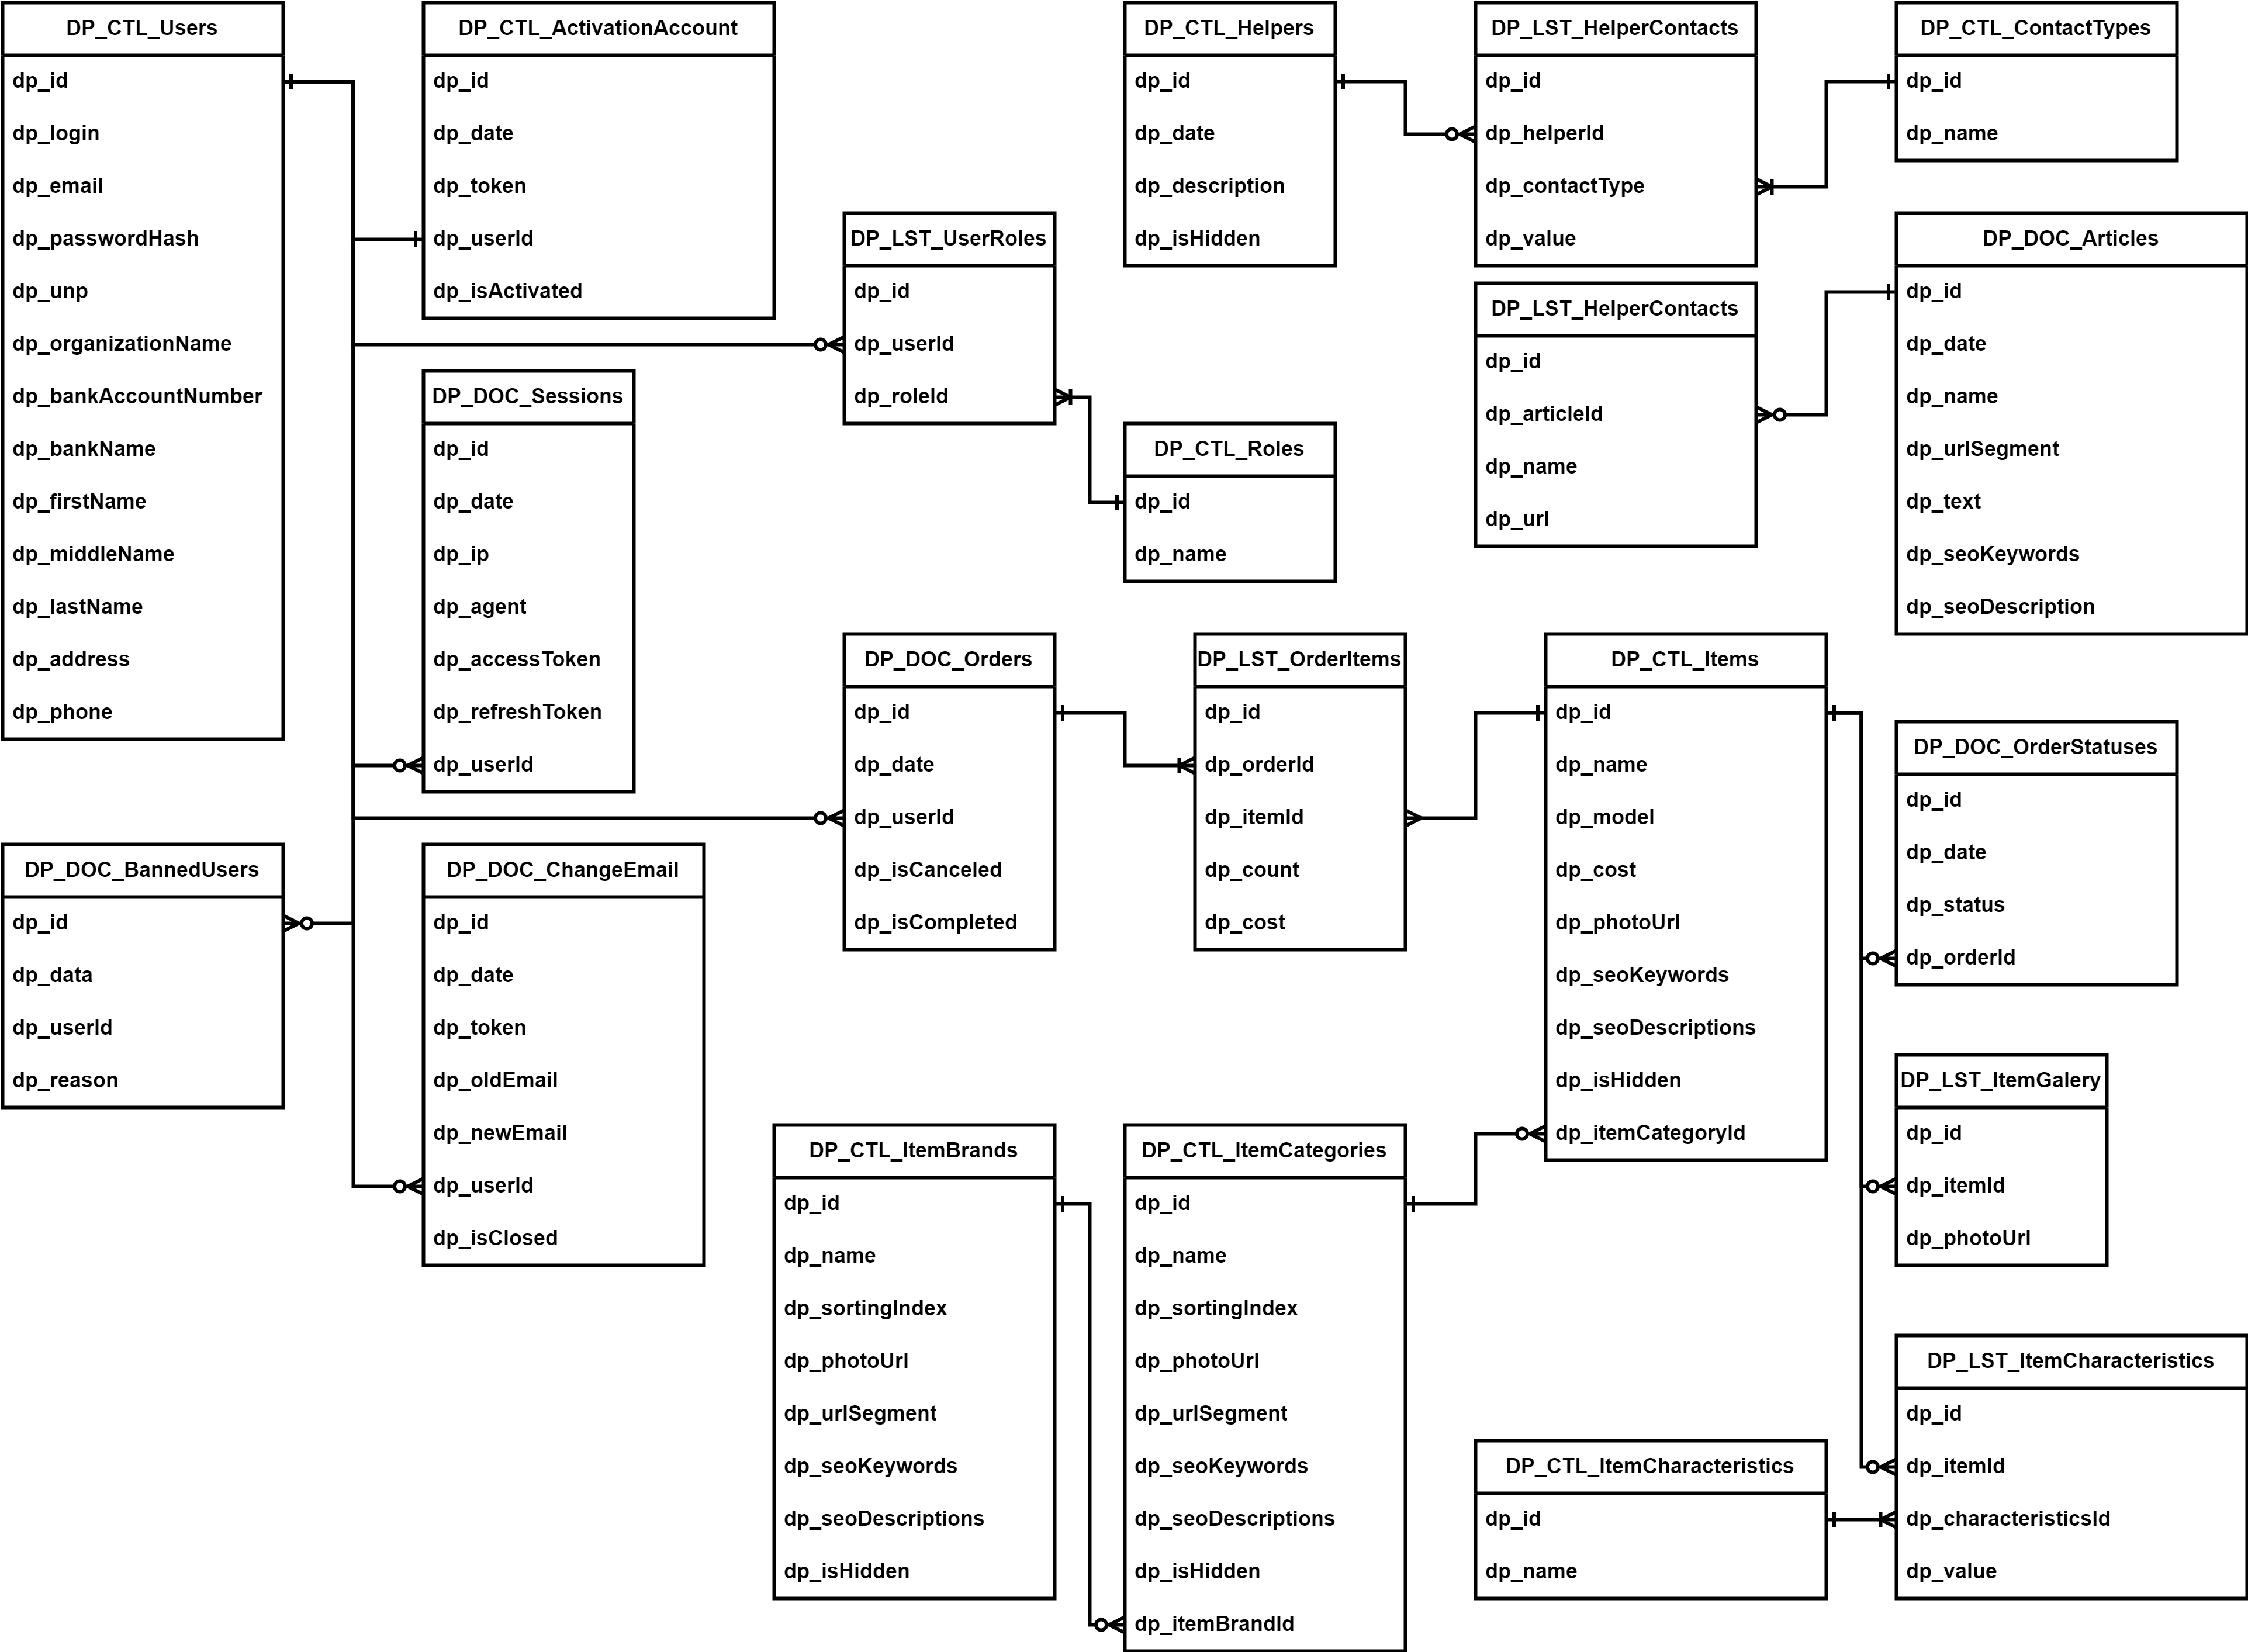
\includegraphics[angle=90, width=18cm]
    {images/db/db.png}

    \caption{Логическая модель}

    \label{fig:db_logic_model}
\end{figure}
